\documentclass[14pt,fleqn]{extarticle}
\usepackage[T2A,T1]{fontenc}
\usepackage[utf8]{inputenc}
\usepackage[russian]{babel}
\usepackage{amsmath}
\usepackage{graphicx}
\usepackage{tabularx}
\usepackage{boldline}
\usepackage{makecell}
\usepackage{arydshln}
\usepackage{mathtools}
\usepackage[a4paper, total={6.5in, 9.5in}]{geometry}

\graphicspath{ {./images/} }
\setlength{\mathindent}{0pt}
\setlength\parindent{0pt}


\begin{document}
	\begin{titlepage}
		
\includegraphics[scale=0.12]{logo}
		\begin{center}
			\textbf{МИНОБРНАУКИ РОССИИ}\\
			\vspace{0.2cm}
			\textbf{Федеральное государственное бюджетное образовательное учреждение высшего образования}\\
			\textbf{«САНКТ-ПЕТЕРБУРГСКИЙ ГОСУДАРСТВЕННЫЙ ЭКОНОМИЧЕСКИЙ УНИВЕРСИТЕТ»}\\
			\vspace{0.6cm}
			Факультет информатики и прикладной математики\\
			Кафедра прикладной математики и экономико-математических методов\\
			\vspace{1cm}
			\textbf{ОТЧЁТ}\\
			по дисциплине:\\
			\textbf{«Теория и системы поддержки принятия решений»}\\
			на тему:\\
			\textbf{«Многокритериальная оптимизации на конечном множестве альтернатив. Задание 2»}\\
		\end{center}
		\vspace{1cm}
		Направление: 01.03.02\\
		Обучающийся: Бронников Егор Игоревич\\
		Группа: ПМ-1901\\
		\vfill
		\begin{center}
			Санкт-Петербург\\
			2022\\
		\end{center}
	\end{titlepage}
	
	\section*{Задача 6}
	\textit{Задание:} Задать критерий для каждого пункта, указанного в заголовке таблицы, и упорядочить банки в соответствии с принятыми критериями (тестами)\\
	
	Из всех факторов (признаков) было решено оставить 10 субъективновыбранных:
	\begin{enumerate}
		\item Максимальная ставка по кредиту, \% $-$ P1 $\leq$ 11.5
		\item Первый взнос, \% $-$ P2 $\leq$ 10
		\item Комиссия банка, \% $-$ P3 $\leq$ 2
		\item Рассмотрение заявки, дн. $-$ P4 $\leq$ 10
		\item Максимальная сумма кредита, млн. руб $-$ P5 $\geq$ 13
		\item Средняя ставка по кредиту, \% $-$ P6 $\leq$ 10
		\item Плата за просрочку, \% $-$ P7 $\leq$ 0.75
		\item Максимальный возраст заёмщика, г. $-$ P8 $\geq$ 60
		\item Максимальный срок кредита, г. $-$ P9 $\geq$ 25
		\item Минимальный общий стаж, г. $-$ P10 $\leq$ 1
	\end{enumerate}
	\newpage
	\begin{center}
		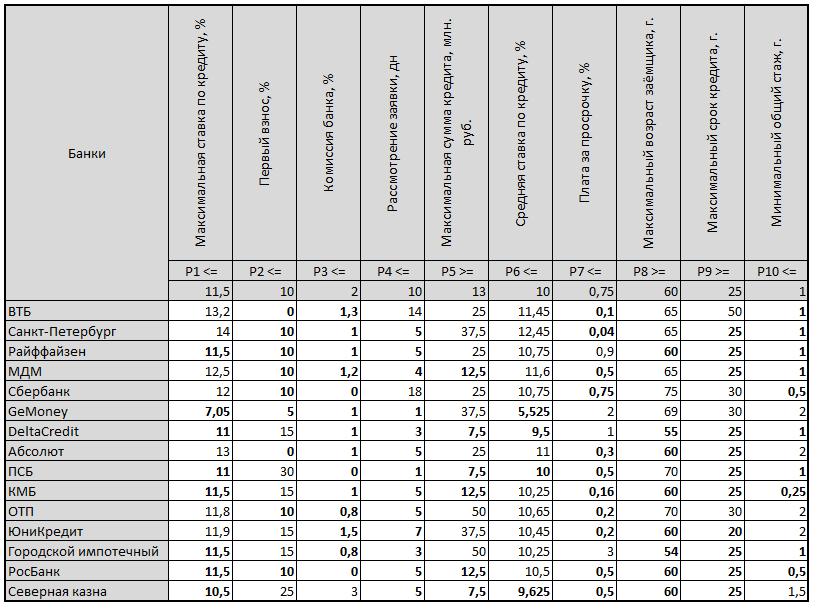
\includegraphics[scale=0.84]{1}
	\end{center}
	\begin{center}
		\textit{Таблица 1} $-$ Характеристики банков
	\end{center}
	Значения признаков, удовлетворяющие ограничениям, выделены полужирным шрифтом. Заменив эти значения единицами, а значения, не удовлетворяющие ограничениям $-$ нулями, получим двоичную таблицу, отражающую выполеннеи заданных ограничений.
	\begin{center}
		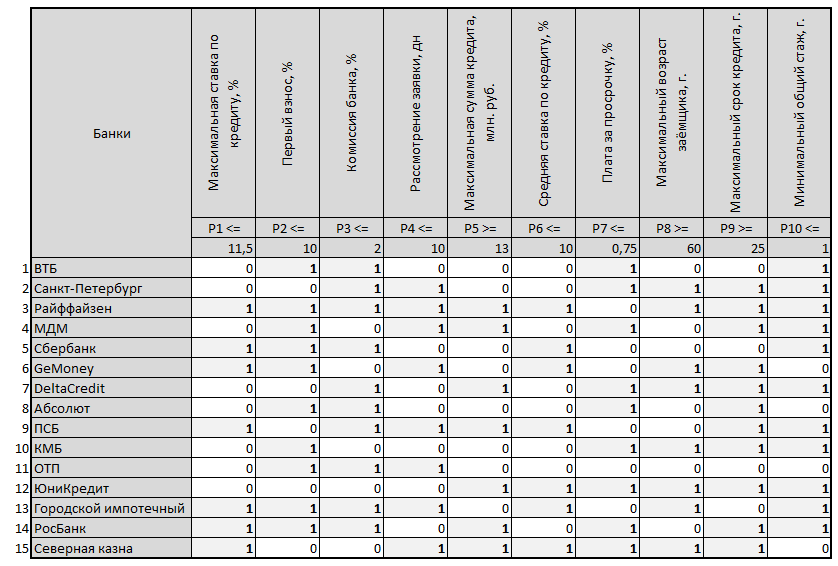
\includegraphics[scale=0.82]{2}
	\end{center}
	\begin{center}
		\textit{Таблица 2} $-$ Оценка свойств банков
	\end{center}
	Воспользуемся оценочной функцией $w_j$ для определения очерёдности критериев в дереве решений:
	\begin{center}
		$w_j = \smashoperator[r]{\sum_{s = 1}^{k_j}}n^0_s n^1_s, \hspace*{1cm} j=\overline{1,n}$
	\end{center}
	, где $n^0_s$ и $n^1_s$ $-$ число нулей и число единиц в $s$-м подмножестве $j$-го уровня, а $k_j$ $-$ число подмножеств на $j$-м уровне.\\
	Результаты вычислений сведены в таблице 3.
	\newpage
	\begin{center}
		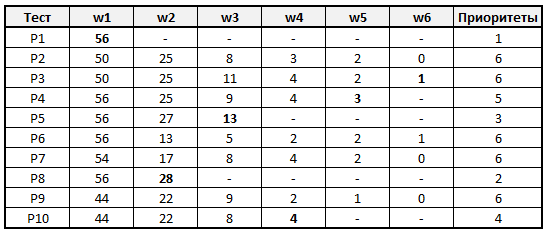
\includegraphics[scale=0.9]{3}
	\end{center}
	\begin{center}
		\textit{Таблица 3} $-$ Определение порядка тестов
	\end{center}
	На основании определения порядка тестов можно построить дерево решений. (\textit{Рисунок 1})
	\begin{center}
		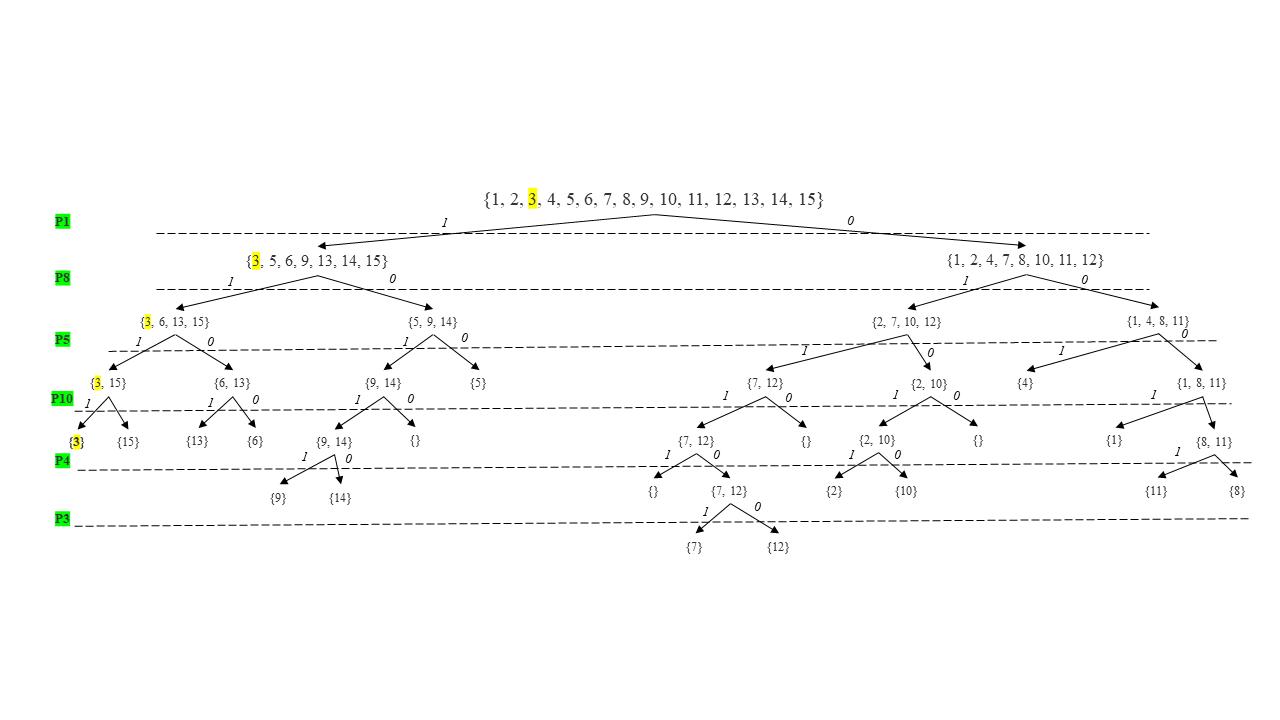
\includegraphics[scale=0.54]{4}
	\end{center}
	\begin{center}
		\textit{Рисунок 1} $-$ Дерево выбора банка
	\end{center}
	Если мы будем идти по левой ветви дерева, то банк который нас удовлетворяет $-$ Райффайзен \{3\}.
	Также данную задачу можно было бы решить и без построения дерева решений. Для этого достаточно в \textit{таблице 3} найти строку с наимбольшим количеством единиц, что означает выполнение максимально возможного количества требований. (\textit{Таблица 4})
	\newpage
	\begin{center}
		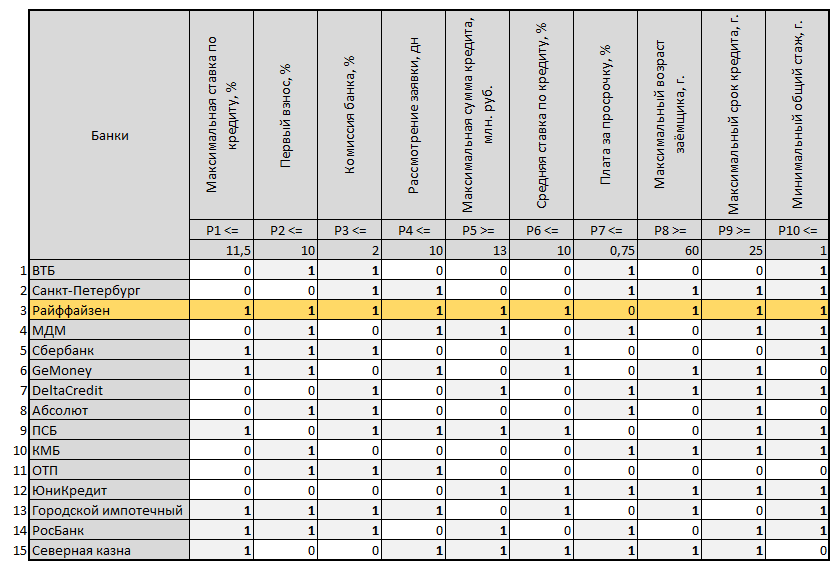
\includegraphics[scale=0.54]{5}
	\end{center}
	\begin{center}
		\textit{Таблица 4} $-$ Выбор банка без дерева решений
	\end{center}
	\textbf{Ответ:} Райффайзен (банк №3)
\end{document}